%\title{Ising Convolutional RBM}
%\author{Emanuel Casiano-Diaz}
%\date{May 18, 2022.}


%Formatting Packages
\documentclass[12pt, two sided]{article}
\usepackage[utf8]{inputenc}
%\usepackage[letter,top=1.1in,bottom=1.1in,left=1.6in,right=1.1in]{geometry}
\usepackage[letterpaper,margin=1in]{geometry}

\usepackage{graphicx}
\usepackage{subfig}
\usepackage{float}

%Math Packages
\usepackage{amsmath}
\usepackage{amssymb}
\usepackage{bm}
\DeclareMathOperator{\Tr}{Tr}

%Physics Package
\usepackage{physics}

%Allow accentuation marks
\usepackage[utf8]{inputenc}
\usepackage[T1]{fontenc}

%Image packages
\usepackage{graphicx}
\graphicspath{ {Images/} }

%Enumerating lists
\usepackage{enumerate}% http://ctan.org/pkg/enumerate

%Adjust depth of subsections
\setcounter{secnumdepth}{3}

%Adjust depth of table of contents
\setcounter{tocdepth}{3}

%References Packages
%\usepackage{biblatex}
%\addbibresource{references.bib}
\usepackage[bookmarks=true]{hyperref}
\hypersetup{
    hidelinks=true,
    linkcolor=blue,
    filecolor=magenta,      
    urlcolor=cyan,
}

%Commands and packages imported from particle entanglement paper
\usepackage{amsmath}
\usepackage{xcolor}
\usepackage{graphicx}
\usepackage{amssymb}

\newcommand{\eket}[1]{\bigl \vert #1 \bigr \rangle}
\newcommand{\R}{\boldsymbol{R}}
\newcommand{\Rt}{\tilde{\R}}
\newcommand{\ebra}[1]{\bigl \langle #1 \bigr \vert}
\newcommand{\eexp}[1]{\bigl \langle #1 \bigr \rangle}
\newcommand{\figref}[1]{Fig.~\ref{#1}}
\renewcommand{\vec}[1]{\boldsymbol{#1}}
\newcommand{\ren}{R\'{e}nyi~}
\newcommand{\rnote}[1]{{\it \textcolor{red}{#1} }}
\newcommand{\Eqref}[1]{Eq.~\eqref{#1}}

%Copied from paper
\usepackage{color}
\usepackage{graphicx}
\usepackage[color=green!60]{todonotes}
\usepackage{physics}
\usepackage{amsthm}
\usepackage{amsmath}
\usepackage{amssymb}
\usepackage{enumerate}
\usepackage{placeins}
\usepackage{booktabs}
\usepackage{dsfont}

%For reference formatting
\usepackage[numbers,sort&compress]{natbib}
\bibliographystyle{nsf_new_url}

\setlength{\footskip}{22pt}

 %Line spacing
\usepackage{setspace}
\doublespace

% --------- Begin Document -------- %
\begin{document}

%----- Introduction -------%

\section{Introduction}

%-----------------------------   Symmetry Implementation ----------------------------------------------% 

\section{Symmetrization implementation}

\subsection{Rotation}

To perform the rotational symmetrization, place the origin at the center of the lattice, then find the groups of vectors with respect to this origin that correspond to $90^\circ$ rotations of each other. 

\begin{figure}[h!]
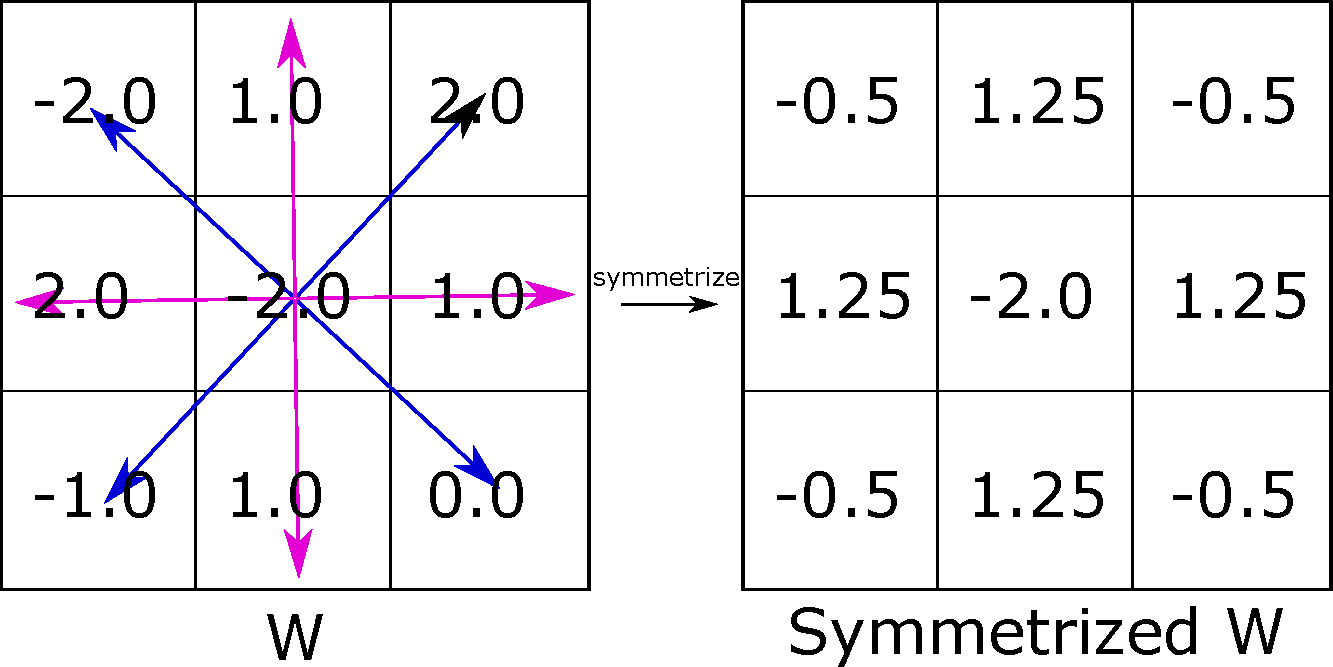
\includegraphics[width=\textwidth]{../figures/symmetrization_diagram.pdf}
\end{figure}

\subsection{Reflection}

To perform the rotational symmetrization, first place a vertical axis through the center of the lattice and take the average of sites that correspond to reflections about this vertical. Then, place a horizontal axis through the center and do the same for the upper and bottom halfs of the lattice.

\begin{figure}[h!]
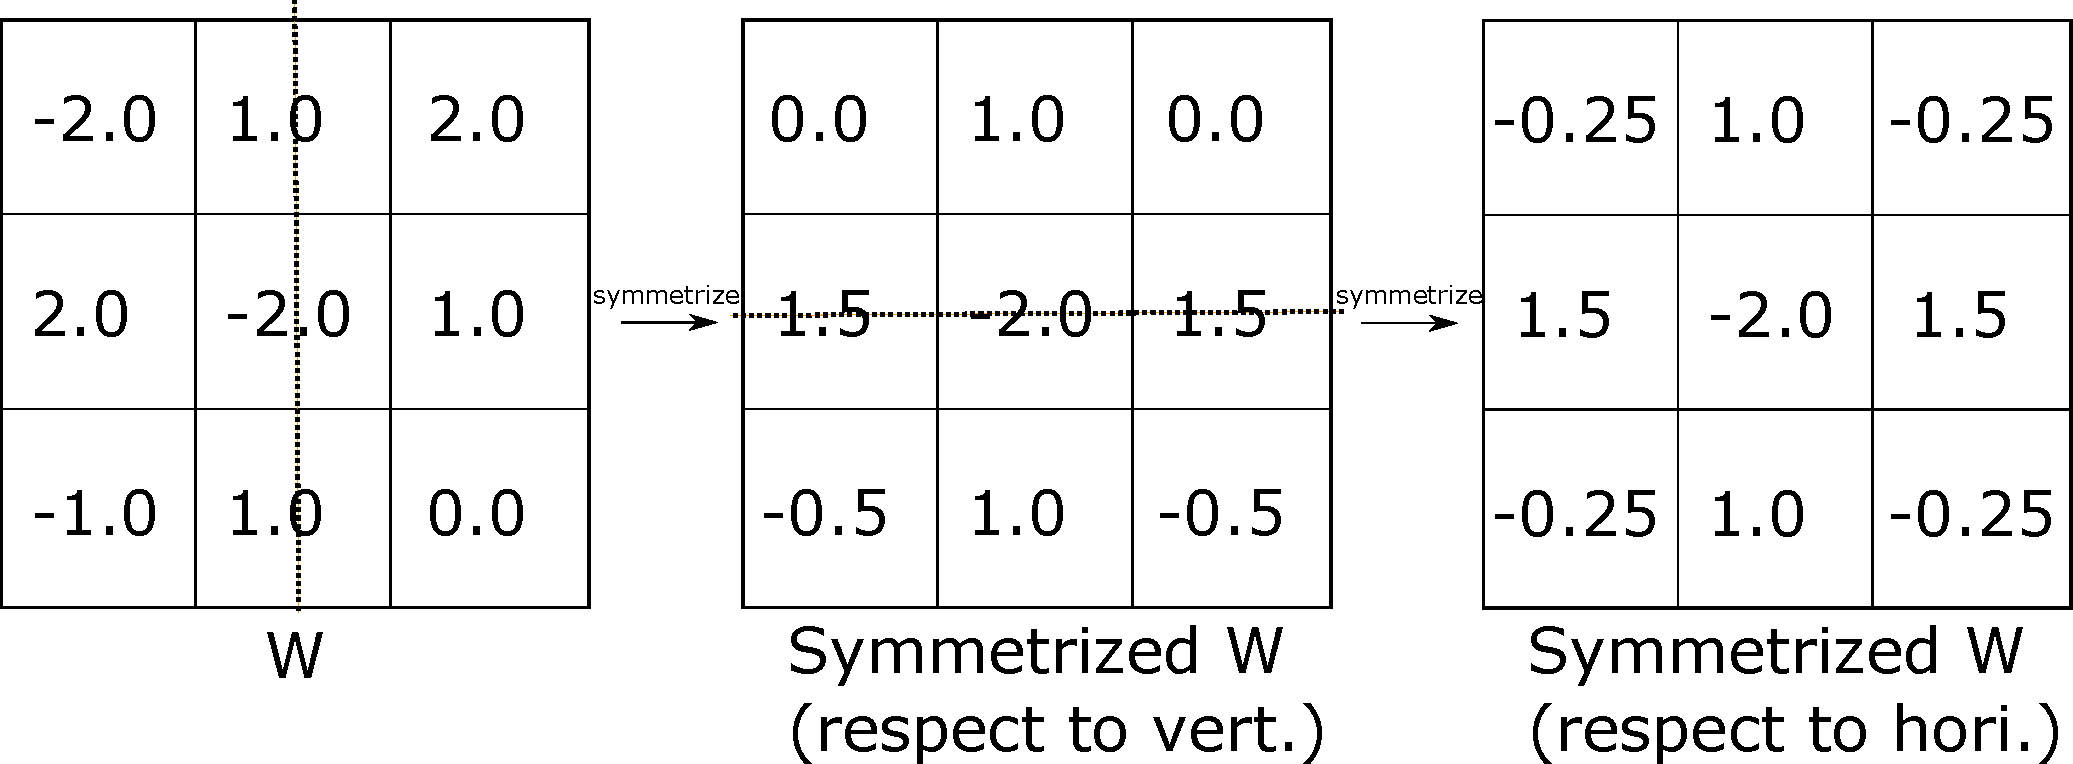
\includegraphics[width=\textwidth]{../figures/reflection_symmetrization.pdf}
\end{figure}


% ------------------------------------------------------ end ---------------------------------- %

% References
\phantomsection 
\addcontentsline{toc}{chapter}{References} 
%\bibliographystyle{apalike} %acm, ieetr, apalike...
 %\section*{Referencess
 \singlespacing
\bibliography{references}

\doublespacing

\end{document}
